\documentclass[11pt,a4paper]{article}
\usepackage[utf8]{inputenc}
\usepackage{amsmath,amssymb}
\usepackage{mathptmx}
\usepackage[left=18mm,right=18mm,top=18mm,bottom=18mm]{geometry}
\usepackage{array,enumitem,fancyhdr}
\usepackage{tikz}
\usetikzlibrary{arrows.meta}

\setlength{\parindent}{0pt}
\setlength{\parskip}{3pt}
\setlist[enumerate]{label=\textbf{(\alph*)},leftmargin=7mm,
  labelsep=2mm,itemsep=4pt,topsep=3pt,parsep=0pt}
\newcommand{\judulsoal}[2]{%
  \par\addvspace{9pt}\hrule height 0.7pt
  \vspace{3pt}\textbf{SOAL #1\quad(25 poin)\quad---\quad #2}\par
  \vspace{2pt}\hrule height 0.7pt\vspace{4pt}}
\newcommand{\judulsolusi}[2]{%
  \par\bigskip\textbf{SOAL #1 --- #2}\par\smallskip}

\pagestyle{fancy}
\fancyhf{}
\renewcommand{\headrulewidth}{0pt}
\fancyfoot[C]{\small Kalkulus 1 (SM224101) $\cdot$ Pembahasan Quiz 1
  \quad---\quad Halaman \thepage}
\fancypagestyle{soal}{%
  \fancyhf{}
  \fancyfoot[C]{\small Kalkulus 1 (SM224101) $\cdot$ Quiz 1
    \quad---\quad Halaman 1 dari 1}}

\begin{document}
\thispagestyle{soal}
\begingroup
\fontsize{11}{13.5}\selectfont
\setlist[enumerate]{label=\textbf{(\alph*)},leftmargin=7mm,
  labelsep=2mm,itemsep=7pt,topsep=5pt,parsep=0pt}
\setlength{\abovedisplayskip}{5pt}
\setlength{\belowdisplayskip}{5pt}

\begin{center}
  \textbf{KALKULUS 1 --- Kode MK: SM224101 (3 SKS, Semester 1)}\\[3pt]
  {\Large\textbf{QUIZ 1}}
\end{center}
\vspace{-5pt}
{\renewcommand{\arraystretch}{1.18}
  \begin{tabular}{|>{\bfseries}p{39mm}|p{\dimexpr\textwidth-39mm-4\tabcolsep-3\arrayrulewidth\relax}|}
    \hline
    Mata Kuliah    & Kalkulus 1 (SM224101), Kelas 3 \\ \hline
    Waktu          & 90 menit                       \\ \hline
    Sifat          & Tutup buku                     \\ \hline
    Dosen Pengampu & Bandung Arry Sanjoyo           \\ \hline
    Hari/Tanggal   & 28 September 2026              \\ \hline
  \end{tabular}}

\judulsoal{1}{Pertidaksamaan \& Nilai Mutlak}
\begin{enumerate}
  \item Selesaikan pertidaksamaan berikut dengan memecahnya menjadi kasus berdasarkan definisi nilai mutlak, lalu nyatakan himpunan penyelesaiannya dalam notasi interval.
        \[
          |3x-5|\le 5x+1
        \]
  \item Selesaikan pertidaksamaan $|x-5|<7$, nyatakan himpunan penyelesaiannya, dan interpretasikan secara geometris (pada garis koordinat) arti dari pertidaksamaan tersebut.
\end{enumerate}

\judulsoal{2}{Grafik Persamaan, Garis, Jarak, Lingkaran \& Parabola}
Diketahui titik $A(2,-3)$ dan $B(5,12)$.
\begin{enumerate}
  \item Tentukan kemiringan garis $AB$, kemudian tulis persamaan garis $AB$ dalam (i) bentuk kemiringan--potongan ($y=mx+b$) dan (ii) bentuk umum ($Ax+By+C=0$).
  \item Tentukan jarak antara titik $A$ dan $B$, serta koordinat titik tengah ruas garis $AB$.
  \item Diberikan persamaan lingkaran $x^2+y^2-8x+2y-8=0$.
        Ubah persamaan tersebut ke dalam bentuk baku dengan cara melengkapkan kuadrat, kemudian tentukan pusat dan jari-jari lingkaran.
  \item Untuk fungsi kuadrat $y=x^2-4x+3$, tentukan:
        (i) koordinat puncak; (ii) titik potong dengan sumbu-$x$ dan sumbu-$y$;
        (iii) sketsa grafiknya pada bidang koordinat di bawah ini;
        (iv) himpunan nilai $x$ yang membuat $y<0$.
\end{enumerate}

\judulsoal{3}{Fungsi \& Operasi pada Fungsi}
Diketahui $f$ dan $g$ sebagai berikut:
\[
  \boldsymbol{f(x)=\sqrt{x+1}}
  \qquad\textbf{dan}\qquad
  \boldsymbol{g(x)=\frac{x+2}{x-3}}.
\]
\begin{enumerate}
  \item Tentukan rumus $(f+g)(x)$ beserta domain $f+g$.
  \item Tentukan hasil operasi $(f\circ g)(x)$ dan $(g\circ f)(x)$ beserta domainnya.
\end{enumerate}

\judulsoal{4}{Grafik Fungsi \& Fungsi Invers}
Diketahui $f(x)=(2x+3)/(x-2)$, $x\ne2$.
\begin{enumerate}
  \item Tentukan titik potong grafik $f$ dengan sumbu-$x$ dan sumbu-$y$.
        Sketsa grafik pada bidang koordinat.
  \item Tentukan rumus $f^{-1}(x)$ beserta domain dan range-nya.
  \item Gambar grafik $f^{-1}$ pada bidang koordinat yang sama,
        nyatakan hubungan antara grafik $f$ dan grafik $f^{-1}$,
        serta hitung nilai $f^{-1}(5)$.
\end{enumerate}
\endgroup

\newpage
\begin{center}
  \textbf{\Large PEMBAHASAN QUIZ 1}
\end{center}

\judulsolusi{1}{Pertidaksamaan \& Nilai Mutlak}
\begin{enumerate}
  \item Nilai mutlak bergantung pada tanda bilangan di dalamnya.
        Jika bilangan itu tak negatif, nilainya tetap.
        Jika negatif, tandanya dibalik.
        Batas kedua kasus diperoleh dari $3x-5=0$, yaitu $x=\frac53$.
        Maka
        \[
          |3x-5|=
          \begin{cases}
            3x-5,  & x\ge\frac53, \\
            -3x+5, & x<\frac53.
          \end{cases}
        \]
        \textbf{Kasus 1: $x\ge\frac53$.}
        Pada daerah ini, $|3x-5|=3x-5$.
        Substitusikan ke pertidaksamaan:
        \begin{align*}
          3x-5 & \le5x+1,                               \\
          -5-1 & \le5x-3x,                              \\
          -6   & \le2x\quad\Longrightarrow\quad x\ge-3.
        \end{align*}
        Hasil ini harus memenuhi syarat kasus, yaitu $x\ge\frac53$.
        Karena setiap $x\ge\frac53$ juga memenuhi $x\ge-3$, irisannya adalah
        $[\frac53,\infty)$.

        \textbf{Kasus 2: $x<\frac53$.}
        Pada daerah ini, $|3x-5|=-(3x-5)=-3x+5$.
        Jadi,
        \begin{align*}
          -3x+5 & \le5x+1,                                    \\
          5-1   & \le5x+3x,                                   \\
          4     & \le8x\quad\Longrightarrow\quad x\ge\frac12.
        \end{align*}
        Gabungkan dengan syarat $x<\frac53$.
        Hasil kasus kedua adalah $\frac12\le x<\frac53$, atau $[\frac12,\frac53)$.

        Setiap solusi cukup memenuhi salah satu kasus.
        Karena itu, ambil gabungan kedua hasil:
        \[
          \boxed{\mathrm{HP}=\left[\frac12,\frac53\right)
          \cup\left[\frac53,\infty\right)
          =\left[\frac12,\infty\right)}.
        \]
        Titik $\frac12$ termasuk karena menghasilkan kesamaan pada pertidaksamaan semula.
        Memang, $|3(\frac12)-5|=\frac72$ dan $5(\frac12)+1=\frac72$.

  \item Nilai $|x-5|$ menyatakan jarak titik $x$ dari titik $5$.
        Agar jaraknya kurang dari $7$, nilai $x-5$ harus berada di antara $-7$ dan $7$.
        Ini sesuai sifat $|u|<a\iff-a<u<a$ untuk $a>0$.
        \[
          |x-5|<7\iff-7<x-5<7.
        \]
        Tambahkan $5$ pada ketiga bagian pertidaksamaan:
        \[
          -7+5<x-5+5<7+5\iff-2<x<12.
        \]
        Jadi, himpunan penyelesaiannya adalah
        \[
          \boxed{\mathrm{HP}=\{x\in\mathbb{R}\mid-2<x<12\}=(-2,12)}.
        \]
        Batas kiri adalah $5-7=-2$ dan batas kanan adalah $5+7=12$.
        Kedua batas tidak termasuk karena jaraknya dari $5$ tepat $7$.
        Pada garis koordinat, tandai keduanya dengan lingkaran kosong.
        Daerah di antaranya merupakan himpunan solusi.

        \begin{center}
          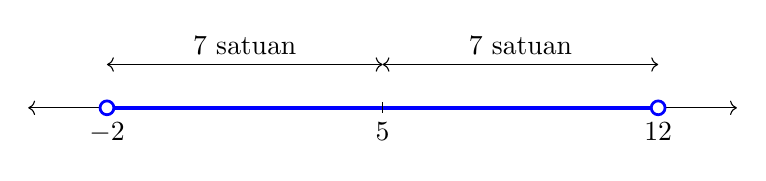
\begin{tikzpicture}[x=0.5cm,y=1cm]
            \draw[<->] (-4,0)--(14,0);
            \draw[blue,line width=1.5pt] (-2,0)--(12,0);
            \foreach \x in {-2,5,12} {
                \draw (\x,0.07)--(\x,-0.07);
                \node[below] at (\x,-0.07) {$\x$};
              }
            \draw[blue,fill=white,line width=1pt] (-2,0) circle (2.5pt);
            \draw[blue,fill=white,line width=1pt] (12,0) circle (2.5pt);
            \draw[<->] (-2,0.55)--node[above] {$7$ satuan}(5,0.55);
            \draw[<->] (5,0.55)--node[above] {$7$ satuan}(12,0.55);
          \end{tikzpicture}
        \end{center}
\end{enumerate}

\newpage
\judulsolusi{2}{Grafik Persamaan, Garis, Jarak, Lingkaran \& Parabola}
\begin{enumerate}
  \item Kemiringan atau gradien menyatakan perubahan $y$ dibanding perubahan $x$.
        Untuk dua titik $(x_1,y_1)$ dan $(x_2,y_2)$, rumusnya
        $m=\frac{y_2-y_1}{x_2-x_1}$.
        Dengan $A(2,-3)$ dan $B(5,12)$, diperoleh
        \[
          m=\frac{12-(-3)}{5-2}=\frac{15}{3}=\boxed{5}.
        \]
        Selisih koordinat $x$ tidak nol, sehingga gradiennya terdefinisi.
        Selanjutnya, gunakan bentuk titik--gradien $y-y_1=m(x-x_1)$.
        Masukkan gradien $5$ dan titik $A(2,-3)$:
        \begin{align*}
          y-(-3) & =5(x-2), \\
          y+3    & =5x-10,  \\
          y      & =5x-13.
        \end{align*}
        Jadi, bentuk kemiringan--potongannya adalah $\boxed{y=5x-13}$.
        Di sini, $m=5$ dan $b=-13$.

        Untuk memperoleh bentuk umum, pindahkan semua suku ke satu ruas:
        \[
          y=5x-13\iff\boxed{5x-y-13=0}.
        \]
        Sebagai pemeriksaan, titik $B(5,12)$ memenuhi $12=5(5)-13$.

  \item Selisih koordinat kedua titik adalah $\Delta x=5-2=3$ dan
        $\Delta y=12-(-3)=15$.
        Kedua selisih ini menjadi sisi siku-siku pada segitiga penghubung $A$ dan $B$.
        Dengan teorema Pythagoras,
        \begin{align*}
          AB & =\sqrt{(\Delta x)^2+(\Delta y)^2}        \\
             & =\sqrt{3^2+15^2}=\sqrt{9+225}=\sqrt{234} \\
             & =\sqrt{9\cdot26}=\boxed{3\sqrt{26}}.
        \end{align*}
        Titik tengah membagi ruas $AB$ menjadi dua bagian sama panjang.
        Koordinatnya diperoleh dengan merata-ratakan koordinat kedua ujung:
        \[
          M=\left(\frac{2+5}{2},\frac{-3+12}{2}\right)
          =\boxed{\left(\frac72,\frac92\right)}.
        \]

        \newpage
  \item Bentuk baku lingkaran adalah $(x-h)^2+(y-k)^2=r^2$.
        Pusatnya $(h,k)$ dan jari-jarinya $r$.
        Kita ubah persamaan soal ke bentuk ini dengan melengkapkan kuadrat.

        Pindahkan konstanta ke ruas kanan, lalu kelompokkan suku $x$ dan suku $y$:
        \[
          (x^2-8x)+(y^2+2y)=8.
        \]
        Untuk $x^2-8x$, tambahkan $(-8/2)^2=16$ agar menjadi $(x-4)^2$.
        Untuk $y^2+2y$, tambahkan $(2/2)^2=1$ agar menjadi $(y+1)^2$.
        Kedua ruas harus ditambah dengan nilai yang sama:
        \begin{align*}
          (x^2-8x+16)+(y^2+2y+1) & =8+16+1, \\
          (x-4)^2+(y+1)^2        & =25.
        \end{align*}
        Jadi, bentuk bakunya $\boxed{(x-4)^2+(y+1)^2=25}$.
        Karena $y+1=y-(-1)$, pusatnya adalah $\boxed{(4,-1)}$.
        Jari-jarinya $\boxed{r=\sqrt{25}=5}$.

  \item \textbf{Koordinat puncak.}
        Lengkapi kuadrat pada fungsi:
        \[
          y=x^2-4x+3=(x^2-4x+4)-1=(x-2)^2-1.
        \]
        Bentuk $y=(x-h)^2+k$ memiliki puncak $(h,k)$.
        Jadi, puncaknya $\boxed{(2,-1)}$ dan sumbu simetrinya $x=2$.

        \textbf{Titik potong kedua sumbu.}
        Pada sumbu-$x$, nilai $y=0$.
        Faktorkan polinom dengan dua bilangan yang jumlahnya $-4$ dan hasil kalinya $3$:
        \[
          x^2-4x+3=(x-1)(x-3)=0\iff x=1\text{ atau }x=3.
        \]
        Hasil kali nol berarti paling sedikit satu faktor bernilai nol.
        Maka titik potong sumbu-$x$ adalah $\boxed{(1,0)}$ dan $\boxed{(3,0)}$.

        Pada sumbu-$y$, nilai $x=0$, sehingga $y=0^2-4(0)+3=3$.
        Titik potong sumbu-$y$ adalah $\boxed{(0,3)}$.

        \textbf{Sketsa grafik.}
        Koefisien $x^2$ positif, sehingga parabola terbuka ke atas.
        Tandai puncak dan titik potong sumbu, lalu hubungkan dengan kurva yang halus.
        Bagian kiri dan kanan kurva simetris terhadap $x=2$.

        \begin{center}
          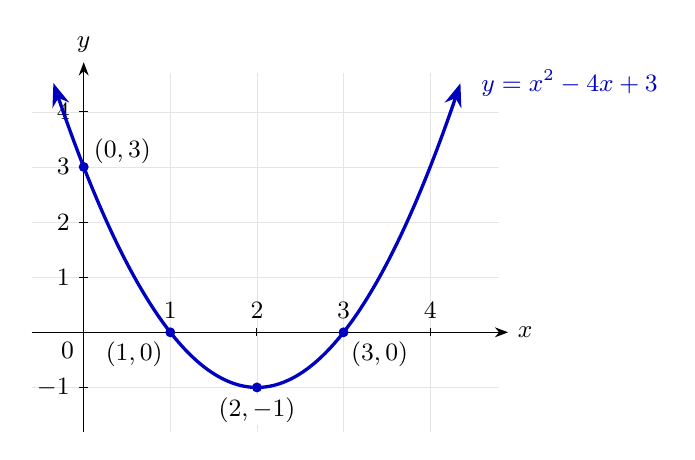
\begin{tikzpicture}[x=1.1cm,y=0.7cm,>=Stealth,font=\small]
            \draw[step=1,gray!20,very thin] (-0.6,-1.8) grid (4.8,4.7);
            \draw[->] (-0.6,0)--(4.9,0) node[right] {$x$};
            \draw[->] (0,-1.8)--(0,4.9) node[above] {$y$};
            \node[below left] at (0,0) {$0$};
            \foreach \x in {1,2,3,4} {
                \draw (\x,-0.07)--(\x,0.07);
                \node[above] at (\x,0.07) {$\x$};
              }
            \foreach \y in {-1,1,2,3,4} {
                \draw (-0.05,\y)--(0.05,\y);
                \node[left] at (-0.05,\y) {$\y$};
              }
            \draw[blue!75!black,very thick,<->,domain=-0.35:4.35,samples=120,smooth]
            plot (\x,{\x*\x-4*\x+3});
            \node[right,blue!75!black,xshift=4pt] at (4.35,4.52) {$y=x^2-4x+3$};
            \foreach \p in {(0,3),(1,0),(2,-1),(3,0)} {
                \fill[blue!75!black] \p circle (1.8pt);
              }
            \node[above right,fill=white,inner sep=1pt] at (0.08,3) {$(0,3)$};
            \node[below left,fill=white,inner sep=1pt] at (0.95,-0.12) {$(1,0)$};
            \node[below right,fill=white,inner sep=1pt] at (3.05,-0.12) {$(3,0)$};
            \node[below,fill=white,inner sep=1pt] at (2,-1.12) {$(2,-1)$};
          \end{tikzpicture}
        \end{center}
        \textbf{Daerah dengan $y<0$.}
        Dari bentuk faktor, syaratnya adalah $(x-1)(x-3)<0$.
        Untuk $1<x<3$, faktor $x-1$ positif dan faktor $x-3$ negatif.
        Hasil kalinya negatif.
        Di luar selang itu, kedua faktor bertanda sama sehingga hasil kalinya positif.
        Jadi, $y<0$ untuk $\boxed{x\in(1,3)}$.
        Kedua batas tidak termasuk karena menghasilkan $y=0$.
\end{enumerate}

\newpage
\judulsolusi{3}{Fungsi \& Operasi pada Fungsi}
\begin{enumerate}
  \item Penjumlahan fungsi dilakukan dengan menjumlahkan nilai $f(x)$ dan $g(x)$
        pada masukan $x$ yang sama.
        Jadi,
        \[
          \boxed{(f+g)(x)=\sqrt{x+1}+\frac{x+2}{x-3}}.
        \]
        Agar jumlah ini dapat dihitung, kedua fungsi harus terdefinisi sekaligus.
        Karena $f(x)$ memuat akar kuadrat, bagian di dalam akar harus tak negatif:
        \[
          x+1\ge0\iff x\ge-1,
          \qquad D_f=[-1,\infty).
        \]
        Pada $g(x)$, penyebut tidak boleh nol:
        \[
          x-3\ne0\iff x\ne3,
          \qquad D_g=\mathbb{R}\setminus\{3\}.
        \]
        Domain jumlah adalah irisan $D_f$ dan $D_g$.
        Artinya, ambil semua $x\ge-1$, kemudian keluarkan $x=3$:
        \[
          \boxed{D_{f+g}=[-1,3)\cup(3,\infty)}.
        \]
        Nilai $-1$ termasuk karena $f(-1)=0$ dan $g(-1)$ terdefinisi.
        Nilai $3$ dikeluarkan karena membuat penyebut $g$ nol.

  \item \textbf{Komposisi $f\circ g$.}
        Pada komposisi ini, hitung $g(x)$ terlebih dahulu.
        Hasilnya dimasukkan ke $f$.
        Karena $f(u)=\sqrt{u+1}$, diperoleh
        \begin{align*}
          (f\circ g)(x) & =f(g(x))=\sqrt{g(x)+1}      \\
                        & =\sqrt{\frac{x+2}{x-3}+1}   \\
                        & =\sqrt{\frac{x+2+x-3}{x-3}}
          =\boxed{\sqrt{\frac{2x-1}{x-3}}}.
        \end{align*}
        Pada langkah penjumlahan, angka $1$ ditulis sebagai $\frac{x-3}{x-3}$.
        Langkah ini berlaku untuk $x\ne3$.

        Ada dua syarat domain.
        Pertama, $g(x)$ harus terdefinisi, sehingga $x\ne3$.
        Kedua, $g(x)$ harus berada dalam domain $f$, yaitu $g(x)\ge-1$.
        Syarat kedua setara dengan
        \[
          g(x)+1\ge0\iff\frac{2x-1}{x-3}\ge0.
        \]
        Pembilang nol saat $x=\frac12$, sedangkan penyebut nol saat $x=3$.
        Kedua titik membagi garis bilangan menjadi tiga selang.
        Tanda pembilang dan penyebut pada tiap selang adalah
        \[
          \begin{array}{c|ccc}
            x                 & (-\infty,\frac12) & (\frac12,3) & (3,\infty) \\ \hline
            2x-1              & -                 & +           & +          \\
            x-3               & -                 & -           & +          \\ \hline
            \dfrac{2x-1}{x-3} & +                 & -           & +
          \end{array}
        \]
        Pecahan tak negatif jika pembilang dan penyebut bertanda sama, atau pembilangnya nol.
        Nilai $x=\frac12$ diperbolehkan karena hasil akarnya nol.
        Nilai $x=3$ tetap dikeluarkan karena penyebutnya nol.
        Jadi,
        \[
          \boxed{D_{f\circ g}=\left(-\infty,\frac12\right]\cup(3,\infty)}.
        \]

        \newpage
        \textbf{Lanjutan soal 3(b): komposisi $g\circ f$.}

        Pada komposisi ini, fungsi $f$ dihitung lebih dahulu.
        Hasilnya menjadi masukan untuk $g$.
        Karena $g(u)=\frac{u+2}{u-3}$, substitusikan $u=f(x)$:
        \[
          (g\circ f)(x)=\frac{f(x)+2}{f(x)-3}
          =\boxed{\frac{\sqrt{x+1}+2}{\sqrt{x+1}-3}}.
        \]
        Agar fungsi dalam terdefinisi, syaratnya $x+1\ge0$, atau $x\ge-1$.
        Selain itu, hasil $f(x)$ harus dapat dimasukkan ke $g$.
        Karena $g$ tidak menerima masukan $3$, kita perlu $f(x)\ne3$.

        Cari nilai $x$ yang membuat penyebut komposisi nol:
        \[
          \sqrt{x+1}-3=0\iff\sqrt{x+1}=3
          \iff x+1=9\iff x=8.
        \]
        Pengkuadratan pada langkah ini sah karena kedua ruas tak negatif.
        Nilai $x=8$ harus dikeluarkan dari domain.
        Jadi, ambil semua $x\ge-1$ kecuali $8$:
        \[
          \boxed{D_{g\circ f}=[-1,8)\cup(8,\infty)}.
        \]
        Batas $-1$ tetap termasuk karena penyebutnya menjadi $0-3=-3$, bukan nol.
        Perhatikan bahwa syarat kedua komposisi berbeda.
        Pada $f\circ g$, keluaran $g$ harus memenuhi syarat akar milik $f$.
        Pada $g\circ f$, keluaran $f$ harus menghindari penyebut nol milik $g$.
\end{enumerate}

\newpage
\judulsolusi{4}{Grafik Fungsi \& Fungsi Invers}
\begin{enumerate}
  \item \textbf{Titik potong sumbu-$x$.}
        Titik pada sumbu-$x$ memiliki koordinat $y=0$.
        Maka kita selesaikan $f(x)=0$.
        Pecahan bernilai nol jika pembilangnya nol dan penyebutnya tidak nol:
        \[
          \frac{2x+3}{x-2}=0\iff2x+3=0\iff2x=-3\iff x=-\frac32.
        \]
        Pada $x=-\frac32$, penyebutnya $-\frac32-2=-\frac72\ne0$.
        Jadi, titik potongnya sah, yaitu $\boxed{(-\frac32,0)}$.

        \textbf{Titik potong sumbu-$y$.}
        Titik pada sumbu-$y$ memiliki koordinat $x=0$.
        Substitusikan nilai itu:
        \[
          f(0)=\frac{2(0)+3}{0-2}=\frac{3}{-2}=-\frac32.
        \]
        Jadi, titiknya $\boxed{(0,-\frac32)}$.

        \textbf{Bentuk grafik dan asimtot.}
        Untuk memudahkan sketsa, pisahkan fungsi menjadi konstanta dan pecahan:
        \[
          f(x)=\frac{2x+3}{x-2}
          =\frac{2(x-2)+7}{x-2}=2+\frac7{x-2}.
        \]
        Bentuk ini merupakan grafik $y=\frac7x$ yang digeser $2$ satuan ke kanan
        dan $2$ satuan ke atas.
        Asimtot tegaknya adalah $x=2$.
        Saat $x$ mendekati $2$, penyebut mendekati nol dan besar nilai fungsi meningkat tanpa batas.

        Asimtot mendatarnya adalah $y=2$.
        Untuk $|x|$ yang semakin besar, nilai $\frac7{x-2}$ mendekati nol.
        Akibatnya, nilai $f(x)$ mendekati $2$.

        Jika $x>2$, pecahan $\frac7{x-2}$ positif, sehingga cabang grafik berada di atas $y=2$.
        Jika $x<2$, pecahannya negatif, sehingga cabang grafik berada di bawah $y=2$.
        Sebagai titik bantu, $f(1)=-5$ dan $f(3)=9$.
        Gunakan asimtot dan titik-titik ini untuk membuat dua cabang kurva.
        Sketsa lengkap ditampilkan bersama grafik invers pada bagian (c).

        \newpage
  \item Fungsi invers membalik hubungan masukan dan keluaran.
        Jika $y=f(x)$, inversnya mengembalikan nilai $x$ dari masukan $y$.
        Karena itu, kita nyatakan $x$ dalam bentuk $y$ terlebih dahulu.

        Misalkan $y=\frac{2x+3}{x-2}$, dengan $x\ne2$.
        Kalikan kedua ruas dengan $x-2$, lalu kumpulkan suku yang memuat $x$:
        \begin{align*}
          y(x-2) & =2x+3,                          \\
          xy-2y  & =2x+3,                          \\
          xy-2x  & =2y+3,                          \\
          x(y-2) & =2y+3,                          \\
          x      & =\frac{2y+3}{y-2}\qquad(y\ne2).
        \end{align*}
        Tukar nama variabel $x$ dan $y$ agar masukan invers ditulis sebagai $x$:
        \[
          \boxed{f^{-1}(x)=\frac{2x+3}{x-2}}.
        \]
        \textbf{Domain dan range.}
        Pada fungsi semula, $D_f=\mathbb{R}\setminus\{2\}$ karena penyebut tidak boleh nol.
        Untuk mencari range, gunakan $f(x)=2+\frac7{x-2}$.
        Pecahan ini tidak pernah nol, sehingga $f(x)$ tidak pernah bernilai $2$.

        Setiap nilai $y\ne2$ dapat dicapai.
        Nilai masukannya adalah $x=\frac{2y+3}{y-2}$, seperti hasil perhitungan di atas.
        Masukan ini sah karena $x-2=\frac7{y-2}\ne0$.
        Jadi, $R_f=\mathbb{R}\setminus\{2\}$.
        Perhitungan tersebut juga memberi tepat satu masukan untuk setiap $y\ne2$,
        sehingga inversnya merupakan fungsi.

        Domain invers sama dengan range fungsi semula.
        Range invers sama dengan domain fungsi semula.
        Karena itu,
        \[
          \boxed{D_{f^{-1}}=R_{f^{-1}}=(-\infty,2)\cup(2,\infty)}.
        \]

        \newpage
  \item Setiap titik $(a,b)$ pada grafik $f$ menjadi titik $(b,a)$ pada grafik invers.
        Pertukaran koordinat ini merupakan pencerminan terhadap garis $y=x$.
        Misalnya, titik $(-\frac32,0)$ berubah menjadi $(0,-\frac32)$.
        Kedua titik tersebut memang ada pada grafik $f$.

        Dari bagian (b), rumus $f^{-1}$ sama dengan rumus $f$ dan domainnya juga sama.
        Maka seluruh grafik $f^{-1}$ berimpit dengan grafik $f$.
        Grafik bersama ini simetris terhadap garis $y=x$.
        Asimtot vertikal $x=2$ dan asimtot horizontal $y=2$ saling bertukar saat dicerminkan.

        \begin{center}
          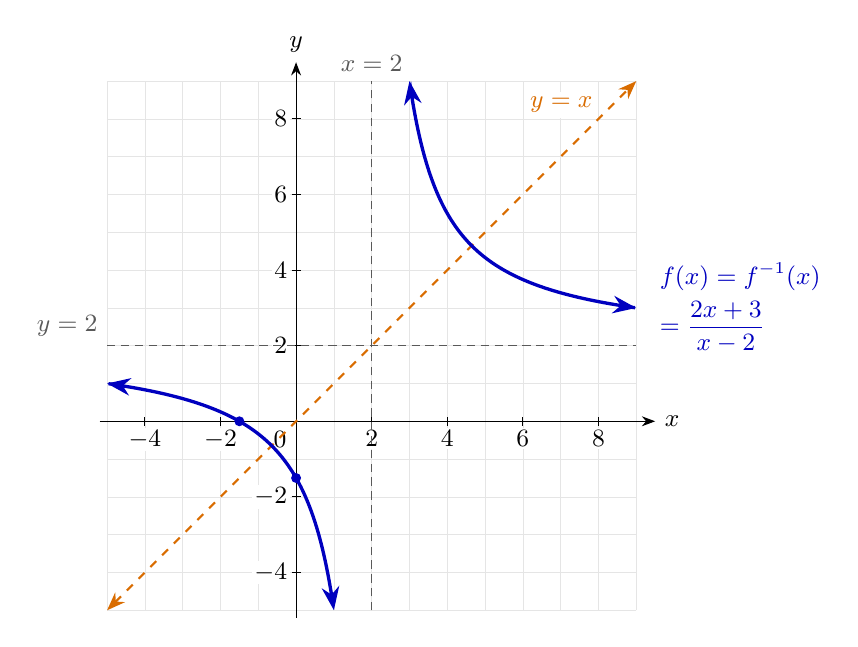
\begin{tikzpicture}[x=0.48cm,y=0.48cm,>=Stealth,font=\small]
            \draw[step=1,gray!20,very thin] (-5,-5) grid (9,9);
            \draw[->] (-5.2,0)--(9.5,0) node[right] {$x$};
            \draw[->] (0,-5.2)--(0,9.5) node[above] {$y$};
            \node[below left] at (0,0) {$0$};
            \foreach \t in {-4,-2,2,4,6,8} {
                \draw (\t,-0.12)--(\t,0.12);
                \node[below,fill=white,inner sep=1pt] at (\t,-0.15) {$\t$};
                \draw (-0.12,\t)--(0.12,\t);
                \node[left,fill=white,inner sep=1pt] at (-0.15,\t) {$\t$};
              }
            \draw[gray!70!black,densely dashed] (2,-5)--(2,9);
            \node[above,gray!70!black] at (2,9) {$x=2$};
            \draw[gray!70!black,densely dashed] (-5,2)--(9,2);
            \node[above left,gray!70!black] at (-5,2) {$y=2$};
            \draw[orange!85!black,thick,dashed,<->,domain=-5:9,samples=2]
            plot (\x,\x);
            \node[above left,orange!85!black,fill=white,inner sep=2pt] at (8,8) {$y=x$};
            \draw[blue!75!black,very thick,<->,domain=-5:1,samples=160,smooth]
            plot (\x,{2+7/(\x-2)});
            \draw[blue!75!black,very thick,<->,domain=3:9,samples=160,smooth]
            plot (\x,{2+7/(\x-2)});
            \node[right,blue!75!black,align=left,xshift=5pt] at (9,3)
            {$f(x)=f^{-1}(x)$\\[3pt]$\displaystyle =\frac{2x+3}{x-2}$};
            \fill[blue!75!black] (-1.5,0) circle (1.8pt);
            \fill[blue!75!black] (0,-1.5) circle (1.8pt);
            % \node[above left,fill=white,inner sep=1pt] at (-1.55,0.15) {$(-\frac32,0)$};
            % \node[below right,fill=white,inner sep=1pt] at (0.15,-1.55) {$(0,-\frac32)$};
          \end{tikzpicture}
        \end{center}
        Untuk menghitung $f^{-1}(5)$, substitusikan $x=5$ ke rumus invers.
        Masukan ini diperbolehkan karena $5\ne2$:
        \[
          f^{-1}(5)=\frac{2(5)+3}{5-2}
          =\frac{10+3}{3}=\boxed{\frac{13}{3}}.
        \]
        Artinya, fungsi semula memetakan $\frac{13}{3}$ ke $5$.
        Kita dapat memeriksanya langsung:
        \[
          f\left(\frac{13}{3}\right)
          =\frac{\frac{26}{3}+3}{\frac{13}{3}-2}
          =\frac{\frac{35}{3}}{\frac73}=5.
        \]
\end{enumerate}

\end{document}
